\texttt{ToDo: Describe the results of the experiments}

%========================================
%===
%=== Principal components analyse (PCA)
%===
%========================================
\subsection{Principal components analyse (PCA)} \label{sss:pca_analyse}
\texttt{ToDo: Describe and document the experiments with PCA}

%========================================
%===
%=== Performance of support vector regression (SVR)
%===
%========================================
\subsection{Performance of support vector regression (SVR)} \label{sss:performance_svr}
Performance of the Multilayer Perceptron is compared against a more commonly used machine learning algorithm, the support vector regression algorithm was chosen as a basis for this comparisons. Henceforth the Support Vector Machine and Support Vector Regression will be shortened to SVM and SVR respectively. Tests of the SVR performance is based on the open source library Libsvm using the Python implementation. Calculations is done using the epsilon-SVM which uses the epsilon intensive loss function. Common parameters used by the SVR are: $\epsilon$ (epsilon) used in the loss function and the cost parameter C.
To give the SVR model a fair chance three different kernels were evaluated: Radial, Sigmoid and Polynomial. These test runs are described in the tables \ref{tab:params_svr_radial}, \ref{tab:params_svr_sigmoid} and \ref{tab:params_svr_poly} of the following subsections. Two different methods of finding the parameters were used, one with manually selected parameters and the other using a genetic algorithm. In the first approach parameter ranges were selected manually in an initial run and with knowledge from that stage a second run was performed with narrowed parameter intervals. Each parameter where tested with about 4-5 points in the interval. The second approach was to let a genetic algorithm select the best parameter set, this procedure is described in details in subsection \ref{sss:ga_tuning}.  

%***
%* Radial Kernel
%***
\subsubsection{Radial Kernel} \label{sss:performance_radial_svr}
The Radial kernel is calculated using the radial basis function (RBF) $e^{-\gamma|u-v|^{2}}$. One kernel parameter $\gamma$ is used.

\begin{table}[H]
\begin{threeparttable}
\begin{tabular}{ | l | l | l | l | l | l | } 
\hline 
Kernel & Run & Param & Low & Hi & Best \\
\hline 
\multirow{21}{*}{Radial} % $e^{-\gamma|u-v|^{2}}$}
& \multirow{7}{*}{Course} & Cost param & 2 & 512 & 256 \\
& & Kernel gamma & 3,051758e-05 & 1,0 & 0,015625 \\  
& & Loss epsilon & 0,000244 & 1,0 & 0,015625 \\ 
\cline{3-6}
& & \multirow{2}{*}{Verify} & \multicolumn{2}{l|}{Error in \%} & 0,040715 \\
& & & \multicolumn{2}{l|}{RMS error} & 0,055867 \\
\cline{3-6}
& & \multirow{2}{*}{Test} & \multicolumn{2}{l|}{Error in \%} & 0,054865 \\
& & & \multicolumn{2}{l|}{RMS error} & 0,073860 \\
\cline{2-6}
& \multirow{7}{*}{Fine} & Cost param & 2,853117 & 4,594973 & 3,797498 \\
& & Kernel gamma & 0,016600 & 0,751315 & 0,111678 \\  
& & Loss epsilon & 0,002039 & 0,092296 & 0,005289 \\
\cline{3-6}
& & \multirow{2}{*}{Verify} & \multicolumn{2}{l|}{Error in \%} & 0,040370 \\
& & & \multicolumn{2}{l|}{RMS error} & 0,055633 \\
\cline{3-6}
& & \multirow{2}{*}{Test} & \multicolumn{2}{l|}{Error in \%} & 0,056366 \\
& & & \multicolumn{2}{l|}{RMS error} & 0,075934 \\
\cline{2-6}
& \multirow{7}{*}{GA} & Cost param & 0,25 & 64 & 5,75 \\
& & Kernel gamma & 0,031250  & 0,156250 & 0,085449 \\  
& & Loss epsilon & 0,003906 & 0,019531 & 0,008057 \\
\cline{3-6}
& & \multirow{2}{*}{Verify} & \multicolumn{2}{l|}{Error in \%} & 0,040241 \\
& & & \multicolumn{2}{l|}{RMS error} & 0,055460 \\
\cline{3-6}
& & \multirow{2}{*}{Test} & \multicolumn{2}{l|}{Error in \%} & 0,056041 \\
& & & \multicolumn{2}{l|}{RMS error} & 0,075436 \\
\hline
\end{tabular}
\begin{tablenotes}
      \small
      \item Radial: $e^{-\gamma|u-v|^{2}}$, GA: population=200, generations=100, selection=50\% X-over=50\%, mutation=5\%
\end{tablenotes}
\caption{Finding parameters for Radial SVR}
\label{tab:params_svr_radial}
\end{threeparttable}
\end{table}


From the table \ref{tab:params_svr_radial} it follows that the lowest verification error are produced by the GA selected parameters giving a RMS error of 0,055460. Applying the test data on this model gives a RMS error of 0,075436 which actually is higher then for the manually selected parameters would have produced.

%***
%* Sigmoid Kernel
%***
\subsubsection{Sigmoid Kernel} \label{sss:performance_sigmoid_svr}
The Sigmoid kernel is calculated using the equation $tanh(\gamma u^{T} v + c_{0})$. Parameters for this kernel are $\gamma$ and the coefficient $c_{0}$.

\begin{table}[H]
\begin{threeparttable}
\begin{tabular}{ | l | l | l | l | l | l | } 
\hline 
Kernel & Run & Param & Low & Hi & Best \\
\hline 
\multirow{24}{*}{Sigmoid} % $tanh(\gamma u^{T} v + c_{0})$}
& \multirow{8}{*}{Course} & Cost param & 789,75 & 1024 & 1024 \\
& & Kernel gamma & 0,000188 & 8 & 0,000244 \\  
& & $coef_{0}$ & 0,001266 & 1 & 0,001953 \\
& & Loss epsilon & 0,013719 & 1 & 0,015625 \\ 
\cline{3-6}
& & \multirow{2}{*}{Verify} & \multicolumn{2}{l|}{Error in \%} & 0,0466276 \\
& & & \multicolumn{2}{l|}{RMS error} & 0,063818 \\
\cline{3-6}
& & \multirow{2}{*}{Test} & \multicolumn{2}{l|}{Error in \%} & 0,062559 \\
& & & \multicolumn{2}{l|}{RMS error} & 0,084042 \\
\cline{2-6}
& \multirow{8}{*}{Fine} & Cost param & 955,59 & 1692,89 & 1692,89 \\
& & Kernel gamma & 0,000367 & 0,000590 & 0,000537 \\  
& & $coef_{0}$ & 0,000865 & 0,001532 & 0,001266 \\
& & Loss epsilon & 0,022095 & 0,032349 & 0,022095 \\
\cline{3-6}
& & \multirow{2}{*}{Verify} & \multicolumn{2}{l|}{Error in \%} & 0,045878 \\
& & & \multicolumn{2}{l|}{RMS error} & 0,062007 \\
\cline{3-6}
& & \multirow{2}{*}{Test} & \multicolumn{2}{l|}{Error in \%} & 0,062063 \\
& & & \multicolumn{2}{l|}{RMS error} & 0,082555 \\
\cline{2-6}
& \multirow{8}{*}{GA} & Cost param & 0,03125 & 7,9688 & 7,8750 \\
& & Kernel gamma & 0,01562 & 1,01562 & 0,01562 \\  
& & $coef_{0}$ & -0,5 & 0,5 & -0,50000 \\
& & Loss epsilon & 0,00098 & 1,0010 & 0,02344 \\ 
\cline{3-6}
& & \multirow{2}{*}{Verify} & \multicolumn{2}{l|}{Error in \%} & 0,044256 \\
& & & \multicolumn{2}{l|}{RMS error} & 0,060323 \\
\cline{3-6}
& & \multirow{2}{*}{Test} & \multicolumn{2}{l|}{Error in \%} & 0,058019 \\
& & & \multicolumn{2}{l|}{RMS error} & 0,078112 \\
\hline
\end{tabular}
\begin{tablenotes}
      \small
      \item Sigmoid: $tanh(\gamma u^{T} v + c_{0})$, GA: population=200, generations=100, selection=50\% X-over=50\%, mutation=5\%
\end{tablenotes}
\caption{Finding parameters for Sigmoid SVR}
\label{tab:params_svr_sigmoid}
\end{threeparttable}
\end{table}

Results from the Sigmoid kernel is obtained in the table \ref{tab:params_svr_sigmoid}. For this kernel the best results, based on the RMS error, are obtained for the model with parameters picked by the GA, with an RMS error of 0,060323 for the verification set and 0,078112 for the test set. This is also the over all lowest error rate. 

%***
%* Polynomial Kernel
%***
\subsubsection{Polynomial Kernel} \label{sss:performance_poly_svr}
For the polynomial kernel the kernel function are; $(\gamma u^{T} v + c_{0})^{d}$. This kernel uses tree parameters: $\gamma$ and the coefficient $c_{0}$ as for the Sigmoid kernel in subsection \ref{sss:performance_sigmoid_svr} and with a additional parameter determining the polynomial degree.

\begin{table}[H]
\begin{threeparttable}
\begin{tabular}{ | l | l | l | l | l | l | } 
\hline 
Kernel & Run & Param & Low & Hi & Best \\
\hline 
\multirow{24}{*}{Poly} % $(\gamma u^{T} v + c_{0})^{d}$}
& \multirow{8}{*}{Course} & Cost param & 0,015625 & 16 & 0,5 \\
& & Kernel gamma & 0,003906 & 0,25 & 0,03125 \\  
& & Kernal degree & 2 & 8 & 8 \\
& & Loss epsilon & 0,007812 & 0,125 & 0,007812 \\ 
\cline{3-6}
& & \multirow{2}{*}{Verify} & \multicolumn{2}{l|}{Error in \%} & 0,0411920 \\
& & & \multicolumn{2}{l|}{RMS error} & 0,0560074 \\
\cline{3-6}
& & \multirow{2}{*}{Test} & \multicolumn{2}{l|}{Error in \%} & 0,0579445 \\
& & & \multicolumn{2}{l|}{RMS error} & 0,077401 \\
\cline{2-6}
& \multirow{8}{*}{Fine} & Cost param & 0,31863 & 1,0 & 0,683013 \\
& & Kernel gamma & 0,022095 & 0,385543 & 0,057309 \\  
& & Kernal degree & 2 & 8 & 5 \\
& & Loss epsilon & 0,003284 & 0,239392 & 0,003284 \\
\cline{3-6}
& & \multirow{2}{*}{Verify} & \multicolumn{2}{l|}{Error in \%} & 0,040356 \\
& & & \multicolumn{2}{l|}{RMS error} & 0,055638 \\
\cline{3-6}
& & \multirow{2}{*}{Test} & \multicolumn{2}{l|}{Error in \%} & 0,056168 \\
& & & \multicolumn{2}{l|}{RMS error} & 0,075729 \\
\cline{2-6}
& \multirow{8}{*}{GA} & Cost param & 0,001 & 4,984375 & 4,140625 \\
& & Kernel gamma & 0,003906 & 1,0 & 0,09375 \\  
& & Kernal degree & 1 & 5 & 3 \\
& & Loss epsilon & 0,001953 & 0,017578 & 0,010986 \\
\cline{3-6}
& & \multirow{2}{*}{Verify} & \multicolumn{2}{l|}{Error in \%} & 0,040886 \\
& & & \multicolumn{2}{l|}{RMS error} & 0,055898 \\
\cline{3-6}
& & \multirow{2}{*}{Test} & \multicolumn{2}{l|}{Error in \%} & 0,058598 \\
& & & \multicolumn{2}{l|}{RMS error} & 0,078522 \\
\hline
\end{tabular}
\begin{tablenotes}
      \small
      \item Poly: $(\gamma u^{T} v + c_{0})^{d}$, GA: population=200, generations=100, selection=50\% X-over=50\%, mutation=5\%
\end{tablenotes}
\caption{Finding parameters for Polygon SVR}
\label{tab:params_svr_poly}
\end{threeparttable}
\end{table}
Results from the tests are in the table \ref{tab:params_svr_poly} where it can be seen that the preferred model based on the RMS error of the verification set originates from the manually fine tuned parameter setting. This selection gives a model that generates a RMS error of 0,075729 when applying the test set.


%========================================
%===
%=== Tuning parameters for the Multilayer Perseptron
%===
%========================================
\subsection{Tuning parameters for the Multilayer Perseptron} \label{sss:tuning_mlp}
In this subsection the process of finding appropriate values for the parameters controlling the calculations generating the prediction model.  
\texttt{ToDo: More stuff...}

%***
%* Finding values for learning rate and momentum
%***
\subsubsection{Finding values for learning rate and momentum} \label{sss:tuning_mlp_learning_momentum}
The importance of how the weights are updated is stressed in subsection \ref{sss:weight_regime} where we introduce the concepts: learning rate and momentum. Here we study the effect of these parameters on the model and determines favourable values these. During this process the MLP configuration is fixed to use two hidden layers with 10 nods each, weight decay is set to $10^{-6}$. In the initial trial the algorithm is allowed to run for 500 iterations. The parameter space for the two parameters are initially tested with the values {0,1 0,3 0,6 0,9} corresponding to the first row of table \ref{tab:first_param_tuning}. 

\begin{table}[H]
\begin{threeparttable}
\begin{tabular}{ | p{1.6cm} | p{1.6cm} | l | l | l | l | l | l | } 
\hline 
\multicolumn{2}{|c|}{Test interval} & \multicolumn{2}{|c|}{Best test result} & \multicolumn{1}{|c|}{Validation error}  & \multicolumn{1}{|c|}{Test error} \\
\hline 
L-rate & Moment & L-rate & Moment & RMS  & RMS  \\
\hline
0,10 - 0,90 & 0,10 - 0,90 & 0,60 & 0,90 & 0,04537 & 0,04840 \\ %--Source=eval30a
\hline
0,10 - 0,70 & 0,90 - 0,90 & 0,70 & 0,90 & 0,04551 & 0,04843 \\ %--Source=eval30b
\hline
0,60 - 0,70 & 0,85 - 0,95 & 0,675 & 0,95 & 0,04417 & 0,04738 \\ %--Source=eval30c
\hline
0,65 - 0,70 & 0,92 - 0,98 & 0,675 & 0,94 & 0,04440 & 0,04735 \\ %--Source=eval30d
\hline
0,66 - 0,68 & 0,94 - 0,96 & 0,68 & 0,95 & 0,04360 & 0,04686 \\ %--Source=eval20e

%L-rate & Moment & L-rate & Moment & Percent & RMS  & Percent & RMS  \\
%\hline
%0,10 - 0,90 & 0,10 - 0,90 & 0,60 & 0,90 & 0,03167 & 0,04537 & 0,03479 & 0,04840 \\ %--Source=eval30a
%\hline
%0,10 - 0,70 & 0,90 - 0,90 & 0,70 & 0,90 & 0,03168 & 0,04551 & 0,03492 & 0,04843 \\ %--Source=eval30b
%\hline
%0,60 - 0,70 & 0,85 - 0,95 & 0,675 & 0,95 & 0,03074 & 0,04417 & 0,03395 & 0,04738 \\ %--Source=eval30c
%\hline
%0,65 - 0,70 & 0,92 - 0,98 & 0,675 & 0,94 & 0,03067 & 0,04440 & 0,03380 & 0,04735 \\ %--Source=eval30d
%\hline
%0,66 - 0,68 & 0,94 - 0,96 & 0,68 & 0,95 & 0,03025 & 0,04360 & 0,03356 & 0,04686 \\ %--Source=eval20e

\hline
\end{tabular}
\begin{tablenotes}
      \small
      \item Average over 5 runs, weight decay = 1e-6, Nodes = [10,10], Iterations = 500, Mini-batch = 194, no noise added
\end{tablenotes}
\caption{Searching for learning rate and momentum using 500 iterations, averages over 5 runs}
\label{tab:first_param_tuning}
\end{threeparttable}
\end{table}
This test indicates that the best parameter setting is located near a momentum of 0,9 and a learning rate near 0,6. After further testing with parameters in the neighbourhood of the favourable values found in the initial test, the best values for the learning rate is 0,68 and for the momentum it is 0,95. The best results for each test is presented in table \ref{tab:first_param_tuning} and is given as the mean of the results from five runs. 
\\
The previous procedure is repeated using 4000 iterations in order to study the effect on the studied parameters. From these tests it is clear that the learning rate has to be reduced to about 0,30 and with the momentum kept fixed. Increasing the number of iterations favours a lower learning rate that avoids ``overfitting'' the model. Results from these tests are gathered in table \ref{tab:first_param_tuning4k}.  

\begin{table}[H]
\begin{threeparttable}
\begin{tabular}{ | p{1.6cm} | p{1.6cm} | l | l | l | l | l | l | } 
\hline 
\multicolumn{2}{|c|}{Test interval} & \multicolumn{2}{|c|}{Best test result} & \multicolumn{1}{|c|}{Validation error}  & \multicolumn{1}{|c|}{Test error} \\
\hline 
L-rate & Moment & L-rate & Moment & RMS & RMS  \\
\hline
0,10 - 0,90 & 0,10 - 0,90 & 0,30 & 0,90 & 0,04227 & 0,04577 \\ %--Source=eval20a
\hline
0,10 - 0,70 & 0,90 - 0,90 & 0,30 & 0,90 &0,04227 & 0,04579 \\ %--Source=eval20b
\hline
0,10 - 0,30 & 0,85 - 0,95 & 0,30 & 0,95 & 0,04185 & 0,04561 \\ %--Source=eval20c
\hline
0,28 - 0,32 & 0,93 - 0,97 & 0,32 & 0,95 & 0,04190 & 0,04576 \\ %--Source=eval20d
\hline
0,31 - 0,33 & 0,96 - 0,98 & 0,32 & 0,98 & 0,04204 & 0,04567 \\ %--Source=eval20e
\hline
0,30 - 0,50 & 0,90 - 0,99 & 0,30 & 0,95 & 0,04181 & 0,04561 \\ %--Source=eval20f

%L-rate & Moment & L-rate & Moment & Percent & RMS  & Percent & RMS  \\
%\hline
%0,10 - 0,90 & 0,10 - 0,90 & 0,30 & 0,90 & 0,02956 & 0,04227 & 0,03247 & 0,04577 \\ %--Source=eval20a
%\hline
%0,10 - 0,70 & 0,90 - 0,90 & 0,30 & 0,90 & 0,02957 & 0,04227 & 0,03250 & 0,04579 \\ %--Source=eval20b
%\hline
%0,10 - 0,30 & 0,85 - 0,95 & 0,30 & 0,95 & 0,02933 & 0,04185 & 0,03234 & 0,04561 \\ %--Source=eval20c
%\hline
%0,28 - 0,32 & 0,93 - 0,97 & 0,32 & 0,95 & 0,02948 & 0,04190 & 0,03249 & 0,04576 \\ %--Source=eval20d
%\hline
%0,31 - 0,33 & 0,96 - 0,98 & 0,32 & 0,98 & 0,02936 & 0,04204 & 0,03246 & 0,04567 \\ %--Source=eval20e
%\hline
%0,30 - 0,50 & 0,90 - 0,99 & 0,30 & 0,95 & 0,02938 & 0,04181 & 0,03242 & 0,04561 \\ %--Source=eval20f

\hline
\end{tabular}
\begin{tablenotes}
      \small
      \item Average over 5 runs, weight decay = 1e-6, Nodes = [10,10], Iterations = 4000, Mini-batch = 194, no noise added
\end{tablenotes}
\caption{Searching for learning rate and momentum using 4000 iterations, averages over 5 runs}
\label{tab:first_param_tuning4k}
\end{threeparttable}
\end{table}
To close up this subsection we found that the best parameters for a long running algorithm are in the neighbourhood of 0,30 for the learning rate and 0,95 for the momentum. For configurations that uses fever iterations to find a suitable model should use values in the vicinity of 0,68 and 0,95 respectively. 


%***
%* Searching for appropriate MLP configuration
%***
\subsubsection{Searching for appropriate MLP configuration} \label{sss:tuning_mlp_nodeconfig}
Configuration of the network has a profound impact on the models performance. In this work the basic configuration of the network is fixed to four layers: input layer with 54 nodes, one for each feature, two hidden layers with configurable number of nodes for each layer and a single output node producing the regression result. In this subsection the challenge is to find a apposite number of nodes for the internal layers of the network. The initial trials are restricted to sixteen nodes for each of the internal layers, see figure \ref{NeuralNet_InHidHidOut}. For this configuration the best result is obtained for the configuration with 14 nodes in the first hidden layer and 8 in the second. As shown in table \ref{tab:node_L1_L2_tuning} the results are quite unvarying with small difference between the best and worst results for the RMS error for the verification set. The low value for the standard deviation for the best configuration is also a sign of a better consistency among those models.    
 
%(eval21a,b,e)}

\begin{table}[H]
\begin{threeparttable}
\begin{tabular}{ | l | l | l | l | l | l | l | l | l | } 
\hline 
\multicolumn{1}{|c|}{} & \multicolumn{2}{|c|}{Test interval} & \multicolumn{2}{|c|}{Result} & \multicolumn{2}{|c|}{Validation error}  & \multicolumn{2}{|c|}{Test error} \\
\hline 
Type & L1 & L2 & L1 & L2 & RMS & S-dev & RMS & S-dev \\
\hline
%4 - 16 & 4 - 16 & 4 & 16 & 16 & 0,04162 & 0,30e-3 & 0,04580 & 0,14e-3 \\ %-Source=eval21a
%\hline
Best & 4 - 16 & 4 - 16 & 14 & 8 & 0,04167 & 0,19e-3 & 0,04554 & 0,20e-3 \\ %-Source=eval21d
\hline
Worst & 4 - 16 & 4 - 16 & 4 & 14 & 0,04315 & 1,25e-3 & 0,04638 & 0,79e-3 \\ %-Source=eval21d
\hline
%20 - 32 & 16 - 32 & 4 & 32 & 24 &  &  &  &  \\ %-Source=eval21b
%\hline
\end{tabular}
\begin{tablenotes}
      \small
      \item Average over 5 runs, weight decay = 1e-6, learning rate = 0,30, momentum = 0,95, Iterations = 4000, Mini-batch = 194, no noise added, regular init 
      %--Source=eval21
\end{tablenotes}
\caption{Searching for node configuration for L1 and L2, averages over 5 runs}
\label{tab:node_L1_L2_tuning}
\end{threeparttable}
\end{table}

The ability to create a high quality model depends on the number of nodes in the network and number of iterations of the algorithm. Results of this investigation is presented in table \ref{tab:node_L1_L2_tuning_iters} where the search for best node configuration from table \ref{tab:node_L1_L2_tuning} has been performed with five different values for the iteration count. As expected increasing the number of iteration generates models which has lower error rate and produces more homogeneous results.  

%(eval21f,g,h)}

\begin{table}[H]
\begin{threeparttable}
\begin{tabular}{ | l | p{0.7cm} | p{0.7cm} | l | p{1.3cm} | p{1.3cm} | p{1.3cm} | p{1.3cm} | } 
\hline 
\multicolumn{1}{|c|}{} & \multicolumn{2}{|c|}{Best result} & \multicolumn{2}{|c|}{Validation error}  & \multicolumn{2}{|c|}{Test error} \\
\hline 
Iterations & L1 & L2 & RMS & S-dev & RMS & S-dev \\
\hline
125 & 4 & 4 & 0,05745 & 3,92e-3 & 0,05937 & 3,71e-3 \\
\hline
250 & 4 & 16 & 0,04930 & 1,47e-3 & 0,05191 & 1,37e-3 \\
\hline
500 & 12 & 8 & 0,04437 & 0,29e-3 & 0,04772 & 0,39e-3 \\
\hline
750 & 12 & 16 & 0,04327 & 0,55e-3 & 0,04673 & 0,24e-3 \\
\hline
1000 & 12 & 8 & 0,04281 & 0,16e-3 & 0,04609 & 0,49e-3 \\
\hline
\end{tabular}
\begin{tablenotes}
      \small
      \item Average over 5 runs, weight decay = 1e-6, Nodes[4-16,4-16], learning rate = 0,30, momentum = 0,95, Mini-batch = 194, no noise added, regular init 
      %--Source=eval21
\end{tablenotes}
\caption{Impact of iteration length on node configuration for L1 and L2, averages over 5 runs}
\label{tab:node_L1_L2_tuning_iters}
\end{threeparttable}
\end{table}

Further conclusions can be drawn from the results in table \ref{tab:node_L1_L2_tuning_iters} where it shows that models with fewer nodes performs better when the number of iterations is low and contrary for models that are permitted more iterations. This is due to the fact that a more complex MLP requires additional iterations to find a good solution. Each new node contributes to the total dimension of the n-dimensional space to search with gradient descent. 

%========================================
%===
%=== Boosting multilayer perceptron performance
%===
%========================================
\subsection{Boosting multilayer perceptron performance} \label{sss:boosting_mlp}
There are several techniques that can improve the results and speed up the running time of the backpropagation algorithm. In this subsection we discuss early stopping that can prevent over fitting of the model, running time can be improved by the weight update regime called mini-batch. Random initialization of the weights and selection of interval can impact which solution is found by the gradient descent algorithm and in the end affect the quality of the models prediction. Finally the concept of conformal prediction is explored, this algorithm predicts a interval in which the result will stay within the given interval with a parametrized likelihood.   


%***
%* Early stopping
%***
\subsubsection{Early stopping} \label{sss:boosting_mlp_stopping}
Early stopping is a regime intended to reduce the problem of over fitting of the model especial if the network has more nodes then actually required to represent the learning problem. One symptom of this is that the the weights start to move away from 0 particularly for the most important nodes. As the training progresses less important weights are also moving away from 0 the training error decreases but the models ability to generalize is reduced. 

\begin{wrapfigure}{R}{0.6\textwidth}
\vspace{-20pt}
\begin{center}
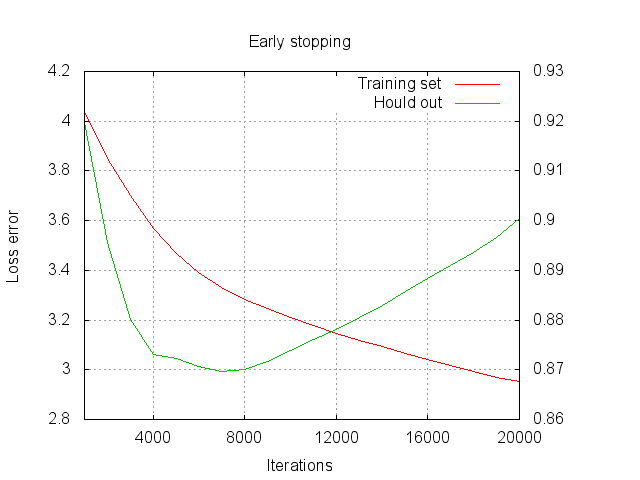
\includegraphics[scale=0.42]{eval24f.png}
\end{center}
\vspace{-20pt}
\caption{Early stopping}
\label{graph:early_stop}
\end{wrapfigure} %-Source=eval24f

The idea behind early stopping is to verify the error rate on a hold out set, in this case the validation set and stop the backpropagation when it increases. This is achieved by monitoring the output of the loss function for the validation data during training. Behaviour of the loss for training and validation sets can be seen in diagram \ref{graph:early_stop}. As long as the loss value decreases the current model are saved and the back propagation continues. If the error on the validation set increases the model are not saved. When the algorithm reaches the predetermined number of iteration the saved model (taken at the lowest seen error rate) is returned as result. So if the error rate decreases asymtotic during the whole backpropagation the final model will be returned if not the intermediary model is used.  
\\

\begin{table}[H]
\begin{threeparttable}
\begin{tabular}{ | l | l | l | l | l | } 
\hline
\multicolumn{1}{|c|}{Testing} & \multicolumn{2}{|c|}{Validation set error}  & \multicolumn{2}{|c|}{Test set error} \\
\hline 
 & Percent & RMS  & Percent & RMS \\
\hline
No early stopping  & 0,03066 & 0,04484 & 0,03306 & 0,04780 \\
\hline
Early stopping & 0,02940 & 0,04154 & 0,03246 & 0,04586 \\
\hline
\end{tabular} 
\begin{tablenotes}
      \small
      \item Average over 5 runs, weight decay = 1e-6, Nodes = [10,10], learning rate = 0,30, momentum = 0,95, Iterations = 50000, Mini-batch = 194, no noise added 
      %--Source=eval124c
\end{tablenotes}
\caption{Early stopping, averages over 5 runns}
\label{tab:early_stop1}
\end{threeparttable}
\end{table}
The result of applying early stopping can be seen in \ref{tab:early_stop1}, here the best result is obtained after about 7000 iterations on average. The favourable effect is significant for both the test and validation set.

%***
%* Mini-batch
%***
\subsubsection{Mini-batch} \label{sss:boosting_mlp_minibatch}
Multilayer Perceptrons can be trained using one of three different schemas discussed in subsection \ref{sss:construction_mlp}. The size of the mini-batch chunks affects the speed of the algorithm, in table \ref{tab:mini_batch1} the algorithm is applied with mini-batch chunks of size 97, 194, 388, 970 and 1940. 

\begin{table}[H]
\begin{threeparttable}
\begin{tabular}{ | l | l | l | l | l | } 
\hline
\multicolumn{1}{|c|}{Testing} & \multicolumn{2}{|c|}{Validation error}  & \multicolumn{2}{|c|}{Runtime} \\
\hline 
Batch size & Percent & RMS error & Running time & Speed up percent\\
\hline
None & 0,02944 & 0,04191 & 159,6 s &  \\
\hline
1940 & 0,02952 & 0,04180 & 129.2 s & 19,0 \\
\hline
970 & 0,02958 & 0,04208 & 91,6 s & 42,6 \\
\hline
388 & 0,02970 & 0,04236 & 81,3 s & 49,0 \\
\hline
194 & 0,02936 & 0,04187 & 78,1 s & 51,0 \\
\hline
97 & 0,02987 & 0,04228 & 75,5 s & 52,7 \\  
\hline
\end{tabular}
\begin{tablenotes}
      \small
      \item Weight decay = 1e-7, Nodes = [10,10], learning rate = 0,30, momentum = 0,95, Iterations = 10000, Early stopping = on, no noise added 
      %--Source=eval25a
\end{tablenotes}
\caption{Mini batch performance, averages over 5 runns}
\label{tab:mini_batch1}
\end{threeparttable}
\end{table}
The rightmost column holds the speed increase of the mini-batch regime over batch processing. As the chunk size of the mini-batch is decreased the root mean square error of the prediction slightly increases due to the fact that fewer samples are used in the calculations that affects the weight update.  

\begin{wrapfigure}{R}{0.6\textwidth}
\vspace{-20pt}
\begin{center}
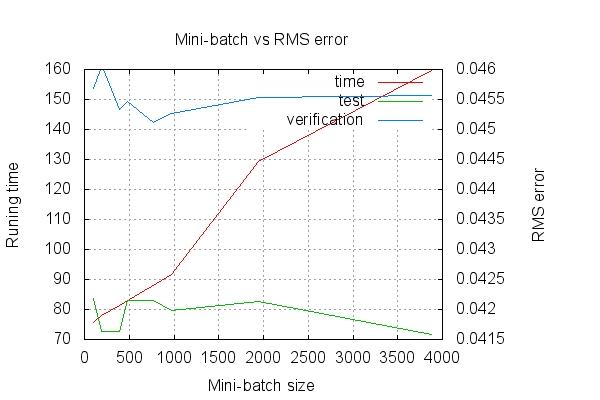
\includegraphics[scale=0.42]{eval25a.png}
\end{center}
\vspace{-20pt}
\caption{Impact of mini-batch size on RMS error}
\label{minibarch_rmsgraph}
\end{wrapfigure}

The results of the tests shows that with a sensible selection of mini-batch chunk size, in this case 970, a good model can be produced in about half the time with a minor increase for the root mean square error.
Studying figure \ref{minibarch_rmsgraph} shows that the RMS error is relatively unaffected by the change of mini-batch size, this behaviour is the same for both the test and verification set. 

\begin{wrapfigure}{R}{0.6\textwidth}
\vspace{-20pt}
\begin{center}
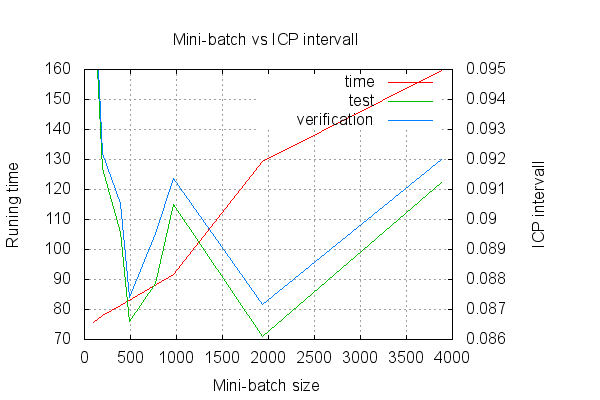
\includegraphics[scale=0.42]{eval25aa.png}
\end{center}
\vspace{-20pt}
\caption{Impact of mini-batch size on ICP-interval}
\label{minibarch_icpgraph}
\end{wrapfigure}

If the ICP interval is taken into account the conditions changes some what. We can see from the figure \ref{minibarch_icpgraph} that a good choice of mini-batch size is 1940 with respect to the performance of the ICP-interval. This gives a speed gain of about 20 percent without increasing the with of the ICP-interval or affects the RMS error significantly. More about the conformal prediction findings in subsection \ref{sss:conformal_prediction}.
\\
In some applications of the MLP processing time is limited due to hardware restrictions or business rules and those gives rise to the mini-batch approach where a good model can be built in a fare amount of time. The total runtime of the model construction can be regulated via the mint-batch size. 


%***
%* Random initialization of weights and dropout
%***
\subsubsection{Random initialization of weights and dropout} \label{sss:boosting_mlp_weight_init}
In this subsection two different schemas for weight initialization are evaluated and the paradigm of ``dropout'' are investigated. 

Initialization of weights are discussed in chapter \ref{sss:glorot_and_bengio} and steams from the work done by Glorot and Bengio in there paper \cite{art}{GlorBeng:10}. The initialization of of the weights is impotent and can have significant effect on the resulting model especial for deep networks. In this work the effect can only be elicited when the noise is added to the weights. When all weights are updated in each iteration the affect of not using the normalized weight initialization is masked by the gradient descent which is still able to find a good solution. This topic is future discussed in chapter \ref{sss:weight_bias_initialization}.

\begin{wrapfigure}{R}{0.6\textwidth}
\vspace{-20pt}
\begin{center}
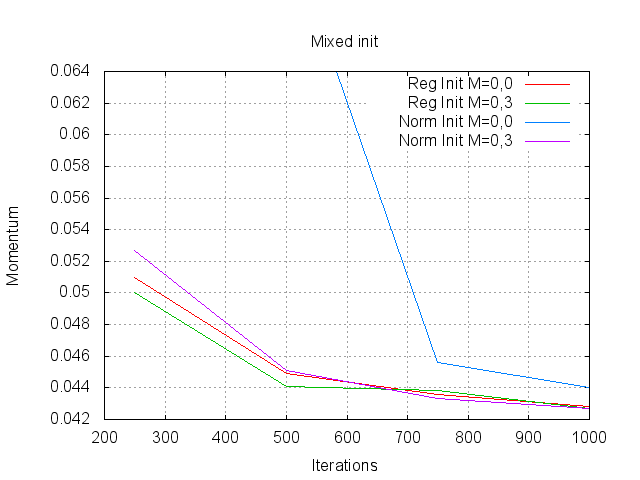
\includegraphics[scale=0.42]{eval33ef.png}
\end{center}
\vspace{-20pt}
\caption{Normalized vs regular initialization}
\label{norm_init}
\end{wrapfigure} %-Source=eval33e, eval33f

The regime of ``dropout'' is discussed in chapter \ref{sss:using_dropout} where the paper \cite{art}{HintSrivKrizSutsSala:12} by Hinton et al. are explored. To investigate the effect five levels of ``dropout'' were tested $\Psi_{M} : M = {0,0 - 0,4}$ (M = proportion of weights left out in weight update), where $\Psi_{0,0}$ corresponds to no ``dropout''.  In diagram \ref{norm_init} the $\Psi_{0,0}, \Psi_{0,3}$ values are presented in conjunction with two weight initialization regimes presented above. From this diagram it can be deduced that ``dropout'' gives an advantage when fewer iteration are used, when the amount of iterations is increased the effect fades out but has clearly a favourable effect for situations where few iteration are used. Future discussions on this topic can be found in chapter \ref{sss:using_dropout}.


%\begin{table}[H]
%begin{threeparttable}
%\begin{tabular}{ | l | l | l | l | l | l | } 
%\hline 
%\multicolumn{2}{|c|}{} & \multicolumn{2}{|c|}{Validation set error}  & \multicolumn{2}{|c|}{Test set error} \\
%\hline 
%Adding noise & Regular init & Percent & RMS  & Percent & RMS \\
%\hline
%\hline
%Yes & Yes & 0,02969 & 0,04226 & 0,03261 & 0,04591 \\
%\hline
%Yes & No & 0,04750 & 0,06595 & 0,05039 & 0,06957 \\
%\hline
%No & Yes & 0,02968 & 0,04216 & 0,03249 & 0,04570 \\
%\hline
%No & No & 0,02998 & 0,04279 & 0,03296 & 0,04652 \\
%\hline
%\end{tabular}
%\begin{tablenotes}
%      \small
%      \item Weight decay = 1e-6, Nodes = 12:6, Iterations = 50000, Early stopping = on, Mini-batch = on, ICP confidence = 95\% 
%      %-Source=eval13b
%\end{tablenotes}
%\caption{Mini batch performance, averages over 4 runns}
%\label{tab:random_initl2}
%\end{threeparttable}
%\end{table}


%***
%* Conformal Prediction
%***
\subsubsection{Conformal Prediction} \label{sss:conformal_prediction}
\texttt{ToDo: More stuff...}

%========================================
%===
%=== Fine tuning of parameters with Genetic Algorithm
%===
%========================================
\subsection{Fine tuning of parameters with Genetic Algorithm} \label{sss:ga_tuning}
Finding appropriate parameters for the Support Vector Regression and the Multilayer Perceptron is a challenge in it self. In article xxxx referred to in xxxx discusses the usage of genetic algorithms to find good parameters. Genetic Algorithms will henceforth often be shortened to GA. The results of the parameter search using a genetic algorithm is presented in the subsection below. A open source package called DEAP (Distributed Evolutionary Algorithms in Python) is used to drive the genetic algorithm in Python. The following parameter configuration was used by the algorithm: a population of 200 individuals running for 100 generations with a selection of 50\%, crossover of 50\%, mutation rate at 5\% and a tournament size of 16. 
\\
\texttt{ToDo: Reference to GA article}

%***
%* Tuning of SVR parameters
%***
\subsubsection{Tuning of SVR parameters} \label{sss:ga_tuning_svr}
The SVR parameters was tuned using a GA previously described. Data from this runns are presented in the tables \ref{tab:params_svr_radial}, \ref{tab:params_svr_sigmoid} and \ref{tab:params_svr_poly} of chapter \ref{sss:performance_svr} and summarised in table \ref{tab:ga_svr_tuning} below.  
\begin{table}[H]
\begin{tabular}{ | l | l | l | l | l |  }
\hline
\multicolumn{1}{|c|}{} & \multicolumn{2}{|c|}{GA tuned} & \multicolumn{2}{|c|}{Manually tuned} \\
\hline
SVR- type & Test error & Test RMS error & Test error & Test RMS error \\
\hline
\hline
Radial & 0,056041 & 0,075436 & 0,056366 & 0,075934 \\
Sigmoid & 0,058019 & 0,078112 & 0,062063 & 0,082555 \\
Polynom & 0,058598 & 0,078522 & 0,056168 & 0,075729 \\
\hline
\end{tabular}
\caption{Tuning of SVR Perseptron using Genetic Algorithm}
\label{tab:ga_svr_tuning}
\end{table}
From the results in table \ref{tab:ga_svr_tuning} it can be seen that no exceptional improvement is gained with the parameters generated using the GA. Performance for the SVR based on a Radial kernel was somewhat better, for the Sigmoid kernel the improvement was the highest in this trial, but the Polynomial kernel performed slightly worse for the model that used GA generated parameters. This vouches for that reasonably good parameters are found and that this results can serve as a good comparison with the results from the MLP. This gives that the MLP has to predict the outcome with a \emph{RMS error below 0,075436} in order to outperform the SVR model. 


%***
%* Tuning of Multilayer Perseptron
%***
\subsubsection{Tuning of Multilayer Perseptron} \label{sss:ga_tuning_mlp}
Inspired from the article \texttt{XXXX} where a GA was used to drive a YYY a GA was constructed to find a good solution to the price estimation problem using a MLP. In this paper we present to different schemas where the optimization is done on two different criteria's. Initially we constructed a GA which goal was to optimize the error in the model. The genome was constructed out of seven parameters used to drive the MLP algorithm, this are presented in table \ref{tab:ga_mlp_genom} together with there range and segment of the genome. 

\begin{table}[H]
\begin{tabular}{ | l | l | l | l | l | l | }
\hline
\multicolumn{1}{|c|}{} & \multicolumn{1}{|c|}{Genom size} & \multicolumn{2}{|c|}{Interval} & \multicolumn{1}{|c|}{} \\
\hline
Parameter & \# bits & Lower & Upper & Winner\\
\hline
Nodes Layer 1 & 6 & 1 & 16 & 16 \\
Nodes Layer 2 & 6 & 1 & 16 & 16 \\
Weight decay & 2 & 1e-5 & 1e-8 & 1e-5 \\
Learning rate & 7 & 0,0078125 & 0,9921875 & 0,15625 \\
Momentum & 7 & 0,0078125 & 0,9921875 & 0,984375 \\
Add noice & 1 & false & true & false \\ 
Regular initialization & 1 & false & true & false \\
\hline
\end{tabular}
\caption{Translation of genome to parameter space}
\label{tab:ga_mlp_genom}
\end{table}

The first unpretentious approach to the task of using a GA to optimize the MLP parameters used the negative RMS error as objective function. Several trials where conducted to find appropriate parameter boundaries for the GA to work with. The results of the MLP models produced by the GA is presented in table \ref{tab:ga_mlp_result}. Here the best and second best results are shown for the three different approaches to MLP optimization. Studying the results from the ingenuous trial to optimize the RMS errors shows that the model produces predictions with a low error but the conformal prediction interval is exceptionally wide, for the best result it is about 0,23 which is almost $\pm$ one quarter of the predicted result. This renders a vain conformal prediction which contributes very little confidence for the model, same situation holds for the second best result.
\\

\begin{table}[H]
\begin{threeparttable}
\begin{tabular}{ | l | l | l | l | l | l | }
\hline
 GA goal & Position &  Set & RMS error & ICP interval & Confidence \\
\hline
\multirow{2}{*}{RMS error}
 & \multirow{2}{*}{first} 
   & Validation & 0,040941 & 0,245985 & 0,969880 \\
 & & Test & 0,044461 & 0,231206 & 0,972864 \\
 \cline{2-6}
 & \multirow{2}{*}{second} 
   & Validation & 0,041765 & 0,180229 & 0,955823 \\
 & & Test & 0,046044 & 0,194983 & 0,965829 \\
 
\hline
 \multirow{2}{*}{ICP} 
 & \multirow{2}{*}{first} 
   & Validation & 0,042136 & 0,073344 & 0,945783 \\
 & & Test & 0,045737 & 0,074467 & 0,928643 \\
 \cline{2-6}
 & \multirow{2}{*}{second} 
   & Validation & 0,042575 & 0,074479 & 0,941767 \\
 & & Test & 0,046370 & 0,075442 & 0,922613 \\

\hline
 \multirow{2}{*}{ICP and RMS} 
 & \multirow{2}{*}{first} 
   & Validation & 0,041491 & 0,069185 & 0,929719 \\
 & & Test & 0,045339 & 0,069497 & 0,910553 \\
 \cline{2-6}
 & \multirow{2}{*}{second} 
   & Validation & 0,041454 & 0,071395 & 0,935743 \\
 & & Test & 0,045476 & 0,071886 & 0,930653 \\
 
\hline
\end{tabular}
\begin{tablenotes}
      \small
      \item GA configuration: population=200, generations=100, selection=50\% X-over=70\%, mutation=5\%
\end{tablenotes}
\caption{Result from MLP model selected by GA}
\label{tab:ga_mlp_result}
\end{threeparttable}
\end{table}

The discouraging results from the first GA trial was tackled by changing the objective function to return the ICP for the MLP model. As shown in the table \ref{tab:ga_mlp_result} this gives more confidence to the model by giving a conformal prediction interval of 0,0754 and meats the 95 percent confidence at 92,26 percent, still with a low RMS error of 0,04637. This result is quite useful but the fact that it only can predict the result within the conformal prediction interval 92,26 percent of the time is still a bit disappointing.
\\
Actually we want to find a good balance between the RMS error and the ICP interval to raise the belief for the model. This is achieved by modifying the objective function to weight the result of the conformal prediction interval ($ICP$) and RMS error ($ERMS$) with there expected values. The resulting objective function becomes $ f_{obj} = \frac{1}{2}\frac{ICP}{ICP_{Expected}} + \frac{1}{2}\frac{ERMS}{ERMS_{Expected}}$. In the previous experiments the MLP used to build the model for the conformal prediction used the same parameters as the MLP for the predicting model. Here the GA is used to select independent parameters for the MLP building the ICP model. We expanding the genome from 24 to 48 bits and using the same parameter transformation described in table \ref{tab:ga_mlp_genom} for the second MLP calculating the results for the ICP. This constellation of perceptrons performs well and constructs a model that can predict the price with a RMS error of 0,0455 and conformal prediction interval of $\pm$0,0719. Though note that the goal of a 95 percent confidence is not reached, the model can only predict results for 93 percent of the test set within the conformal prediction interval. 

\subsection{Summation of results} \label{sss:result_summup}
The thesis in this paper is that apartment prices on the Stockholm market can be predicted with a Multilayer Perceptron. Results from this paper can be compared with the findings from article \cite{art}{MahaBakeNorw:99} discussed in subsection \ref{sss:using_ann} where prediction of the real estate values in the Malaysian hosing market was studied and where they as result obtained a root mean square error of 0,061717 for there MLP based model. This should be compared to the root mean square error of 0,0455 shown in this paper.
To evaluate the performance of the models the results has to be translated to actual denormalizing apartment prices, this is presented in table \ref{tab:result_in_sek} below. 

\begin{table}[H]
\begin{threeparttable}
\begin{tabular}{ | l | l | l | l | l | }
\hline
 Approach & Error & RMS error & ICP interval & Confidence \\
\hline
SVR Radial & 481.000 kr &  647.931 kr  &  &  \\
MLP & 273.000 kr & 356.000 kr & 613.000 kr & 93,6 \% \\
\hline
\end{tabular}
\caption{Result from above experiments}
\label{tab:result_in_sek}
\end{threeparttable}
\end{table}

From table \ref{tab:result_in_sek} we can see that the Multilayer Perceptron outperforms the Support Vector Regression and the the result from the latter is to deficient to be used in many commercial applications. The results from the MLP are more promising and can predict the price with a root mean square error of about 356.000 kr and estimate the prise within a intervall of $\pm$ 613.000 kr 93,6 percent of the time. This precision should be sufficient to be used as a tool or indicator for realtors and consumers. Note that this estimate should be compared with a realtor estimating a price without the ability to visit the apartment or get any description of it expect from the address. In this context the estimate produced by the MLP can probably compete with a experienced estate agents appraise. 


%===========
%=== RMS ===
%===========
%lgh_tan_reg_icp_norm_l2(1e-5,16,16,10000,0.15625,0.984375,true,194,0.95,false,false)
%ICP confidence 0.950000 using 121 examples, index is 6. Alpha: first 603.190851, last 1.244873
%The classification error rate on the training data is 0.028924, rms is 0.040935, mean intervall is 0.233115, std intervall is 0.166695 and hit rate 0.970619
%The classification error rate on the validation data is 0.028550, rms is 0.040941, mean intervall is 0.245985, std intervall is 0.192299 and hit rate 0.969880
%The classification error rate on the test data is 0.031417, rms is 0.044461, mean intervall is 0.231206, std intervall is 0.166147 and hit rate 0.972864

%------

% lgh_tan_reg_icp_norm_l2(1e-5,16,16,10000,0.1875,0.921875,true,194,0.95,false,false)
% ICP confidence 0.950000 using 121 examples, index is 6. Alpha: first 214.069671, last 0.019022
% The classification error rate on the training data is 0.029043, rms is 0.041703, mean intervall is 0.190465, std intervall is 0.179744 and hit rate 0.964948
% The classification error rate on the validation data is 0.029626, rms is 0.041765, mean intervall is 0.180229, std intervall is 0.156340 and hit rate 0.955823
% The classification error rate on the test data is 0.032542, rms is 0.046044, mean intervall is 0.194983, std intervall is 0.198857 and hit rate 0.965829


%============
%=== ICP ===
%============

% lgh_tan_reg_icp_norm_l2(1e-8,14,14,10000,0.640625,0.796875,true,194,0.95,true,true)
% ICP confidence 0.950000 using 121 examples, index is 6. Alpha: first 34.039659, last 0.012978
% The classification error rate on the training data is 0.030181, rms is 0.043669, mean intervall is 0.074349, std intervall is 0.028125 and hit rate 0.937371
% The classification error rate on the validation data is 0.029655, rms is 0.042136, mean intervall is 0.073344, std intervall is 0.028510 and hit rate 0.945783
% The classification error rate on the test data is 0.032503, rms is 0.045737, mean intervall is 0.074467, std intervall is 0.029755 and hit rate 0.928643

%------

% lgh_tan_reg_icp_norm_l2(1e-7,6,14,10000,0.640625,0.796875,true,194,0.95,true,true)
% ICP confidence 0.950000 using 121 examples, index is 6. Alpha: first 67.202414, last 0.171021
% The classification error rate on the training data is 0.029811, rms is 0.043386, mean intervall is 0.074484, std intervall is 0.026782 and hit rate 0.935309
% The classification error rate on the validation data is 0.029856, rms is 0.042575, mean intervall is 0.074479, std intervall is 0.027931 and hit rate 0.941767
% The classification error rate on the test data is 0.033011, rms is 0.046370, mean intervall is 0.075442, std intervall is 0.029506 and hit rate 0.922613

%=============
%=== ICP2 ===
%=============
%lgh_tan_reg_icp_norm_l2XP(1e-5,15,11,10000,0.515625,0.890625,true,194,true,true,1e-6,4,11,10000,0.46875,0.46875,true,194,0.95,true,true)
% ICP confidence 0.950000 using 121 examples, index is 6. Alpha: first 33.389415, last 0.092254
% The classification error rate on the training data is 0.029884, rms is 0.043192, mean intervall is 0.069087, std intervall is 0.023805 and hit rate 0.930155
% The classification error rate on the validation data is 0.029315, rms is 0.041491, mean intervall is 0.069185, std intervall is 0.024511 and hit rate 0.929719
% The classification error rate on the test data is 0.032183, rms is 0.045339, mean intervall is 0.069497, std intervall is 0.025487 and hit rate 0.910553

% -----

%  lgh_tan_reg_icp_norm_l2XP(1e-5,15,11,10000,0.546875,0.96875,true,194,true,true,1e-6,4,11,10000,0.46875,0.453125,true,194,0.95,true,true)
% ICP confidence 0.950000 using 121 examples, index is 6. Alpha: first 92.156758, last 0.209409
% The classification error rate on the training data is 0.028845, rms is 0.041562, mean intervall is 0.072385, std intervall is 0.019951 and hit rate 0.941237
% The classification error rate on the validation data is 0.029079, rms is 0.041454, mean intervall is 0.071395, std intervall is 0.019100 and hit rate 0.935743
% The classification error rate on the test data is 0.031812, rms is 0.045476, mean intervall is 0.071886, std intervall is 0.021123 and hit rate 0.930653




